%=====================================================================
%  分片 G：§4 含物质的 $N=2$ 规范理论的 Seiberg--Witten 分析
%  覆盖原文 PDF 第 65--80 页（§4 标题与导语、§4.1--§4.6，含图 6、图 7）
%=====================================================================

\section{含物质的 $N=2$ 规范理论的 Seiberg--Witten 分析}

\begin{keypoints}
\begin{itemize}
\item \textbf{物理图像：}加入 $N_f$ 个物质超多重态后，库仑分支上除磁单极/双子奇点外还出现夸克变无质量的奇点；奇点位置随裸质量移动，$m_i=0$ 时其数目与电荷由 $R$ 对称性的离散子群和中心荷的变换性质所决定。
\item \textbf{数学工具：}电荷归一化改为 $n_e\to2n_e$、$a\to a/2$，且 $2a_D=\partial{\cal F}/\partial a$；有物质时单值变换成为作用在 $(m/\sqrt2,a_D,a)^T$ 上的 $3\times3$ 矩阵（见原文 PDF 第 72 页），故对偶群一般不再是 $SL(2,Z)$，谱也仅在 $N_f=4$ 时才可能保持 $SL(2,Z)$ 不变。
\item \textbf{关键结论：}无质量各理论的 Seiberg--Witten 曲线为 $N_f=0$：$y^2=x^3-ux^2+\frac14\Lambda^4x$；$N_f=1$：$y^2=x^2(x-u)+t\Lambda_1^6$；$N_f=2$：$y^2=(x^2-\tilde\Lambda_2^4)(x-u)$；$N_f=3$：$y^2=x^2(x-u)+\tilde\Lambda_3^2(x-u)^2$。
\item \textbf{BPS 态：}零裸质量夸克（$SO(2N_f)$ 的矢量）与磁单极（$2N_f$ 个费米子零模生成 $Spin(2N_f)$ 的旋量）满足 $M=\sqrt2\,|Z|$，其中 $Z=n_ea+n_ma_D+S\,m/\sqrt2$；$N_f=1,3$ 时存在宇称简并，$N_f=2,4$ 时没有。
\item \textbf{几何对应：}模空间视为椭圆曲线族 $E_u$ 的模空间，$a,a_D$ 为其周期；判别式零点阶数给出单值变换的指数，$u\to\infty$ 处 $M_\infty=PT^{N_f-4}$，且有限奇点处单值矩阵之积应等于 $M_\infty$。
\end{itemize}
\end{keypoints}

本节我们考虑规范群为 $SU(2)$、并与 $N_f$ 个物质多重态耦合的 $N=2$
超对称规范理论。这一分析牵涉许多技术性问题，理论的性质依赖于 $N_f$
的取值。与通常的 QCD 一样，物质场（费米子）与规范玻色子对 $\beta$
函数的贡献符号相反。因此，为保证渐近自由，我们要求 $N_f
\leq 4$。$N_f =4$ 的理论在微扰论的各阶都是有限的，而且当夸克无质量时，
它极可能在非微扰层次上也是共形不变的。Seiberg 与 Witten
给出了证据，表明这一理论是 $SL(2,Z)$ 不变理论的一个例子。四维中已知的
另一个 $SL(2,Z)$ 不变理论是 $N=4$ 超对称规范理论，它的 $\beta$
函数同样为零。不过，下文我们将主要集中于 $N_f\leq 3$。至于 $N_f=4$
的情形，读者可参阅 Seiberg 与 Witten 的原始工作 \cite{SW2}。

% [Tutor Note: 见原文 PDF 第 65 页导语第一段。原文称“为保证渐近自由要求 $N_f\le4$”，
% 但由式 (111) 可见 $N_f=4$ 时 $\beta(g)=0$：该理论是有限的（共形不变），
% 并非渐近自由；严格的渐近自由条件是 $N_f<4$。此处是原文的宽泛表述，阅读时不要
% 把 $N_f=4$ 当作渐近自由理论。]

有物质存在时，采用一个不同于前几节的电荷归一化会比较方便。在 $N=2$
纯规范理论中，所有场都按伴随表示变换，粒子与磁单极的荷都是整数。因此，
在公式 $Z=a n_e + a_D n_m$ 中，$n_e$ 与 $n_m$ 都是整数。按这一归一化，
一旦引入夸克，$n_e$ 就可能取半整数。本节我们采用一个稍有不同的约定：
为保证 $n_e$ 始终为整数，把它乘以 2，同时把 $a$ 除以 2，以保持质量公式
不变。由于 $a_D$ 保持不变，它现在由 $2 a_D=\partial{\cal F}/\partial a$
给出。用规范不变量 $u={\rm Tr}\phi^2$ 表示，当 $|u|\rightarrow\infty$ 时，
在这一归一化下 $a$ 与 $a_D$ 的渐近行为变为
$$
a \cong \frac{1}{2} \sqrt{2u}\,, \quad
a_D \simeq i \frac{4}{\pi} a \log a\,.
$$

% [Tutor Note: 见原文 PDF 第 65 页。与第 3 节的纯规范归一化对照：那里
% $a\cong\sqrt{2u}$、基本表示的夸克 $n_e=\pm1/2$、$W$ 玻色子 $n_e=\pm1$；
% 本节把 $n_e$ 乘 2、$a$ 除 2，于是 $a\cong\frac12\sqrt{2u}$ 而 $a_D$ 不变
% （$2a_D=\partial{\cal F}/\partial a$）。这个因子 2 贯穿全节，尤其是式
% (113)、第 76 页的换基与式 (115)，核对时最易出错。]

此外，有效耦合也被重新标度为 $\tau=\partial a_D/\partial a = \frac{\theta}{\pi}
+ \frac{8 \pi i}{g^2}$。电荷的这一重新标度会改变确定模型解的曲线形式，
但物理保持不变。

本节我们将研究规范群为 $SU(2)$ 的理论。在这种情况下，最有趣的动力学
出现在模空间的库仑分支上，在那里 $SU(2)$ 破缺为 $U(1)$。因此，先研究
$N = 2$ 超对称 QED 是有启发性的。

\subsection{$N = 2$ 超对称量子电动力学（SQED）}

$N=2$ 超对称 QED 包含光子矢量多重态与 $k$ 个夸克超多重态。光子多重态
由 $N=1$ 手征超场 $(W_{\alpha}, A)$ 组成，每个夸克超多重态由两个 $N=1$
手征超场 $M^i$ 与 $\widetilde M_i$ 组成，它们的 $U(1)$ 荷分别为 $+1$ 与
$-1$。唯一可重整且与 $N = 2$ 相容的超势是：
$$
{\cal W}=\sqrt{2} A M^i\widetilde M_i + \sum_i m_i M^i\widetilde
M_i\,. 
$$

% [Tutor Note: 见原文 PDF 第 66 页。$A$ 是光子矢量多重态的 $N=1$ 手征超场
% （其最低分量为复标量），$W_\alpha$ 是场强手征超场；$M^i$ 与 $\widetilde M_i$
% 的味指标 $i$ 与 $U(1)$ 规范指标都隐含缩并。超势中的 $\sqrt2$ 系数不是可以
% 随意改动的约定：它保证同一超多重态内玻色子与费米子质量简并，并与 BPS 质量
% 公式中的 $\sqrt2$ 相关联。]

当 $m_i = 0$ 时，理论具有整体对称群 $SU(k)\times SU(2)_R \times
U(1)_{\cal R}$。$SU(k)$ 是作用于 $k$ 个超多重态的味对称群，$SU(2)_R$
转动两个超对称，而 $U(1)_{\cal R}$ 是通常的 $R$ 对称性，它受反常的破坏。
与无物质的情形一样，策略是先确定经典模空间，再看量子模空间是否定性不同。
理论的对称性对于确定这些模空间的结构非常有用。

% [Tutor Note: 见原文 PDF 第 66 页。原文 “afflicted by an anomaly” 一语指该整体
% 对称性被瞬子反常破缺（下一小节将具体算出 ${\bf Z}_{4N_c-2N_f}$），并非说它
% 完全不是对称性；故译作“受反常的破坏”，而非“具有反常”。]

一般而言，经典模空间有希格斯分支与库仑分支。希格斯分支由某些 $M^i$
获得真空期望值来定义。在这种情况下，无论在 QED 中还是在规范群为 $SU(2)$
的 QCD 中，规范群都被完全破缺。对 $k=1$，不存在希格斯相。当 $k \geq 2$、
$m_i = 0$ 时，利用整体对称性以及 $D$ 项的消失条件，可以把 $M$ 与
$\widetilde M$ 转到 $M=(B,0,0,...)$ 与 $\widetilde M = (0,
B,0,...)$ 的形式。由此可以读出依赖于味数 $k$ 的各种对称性破缺模式。
处在希格斯分支上的理论不含磁单极或双子，因此其动力学可能性不如库仑分支
丰富。经典模空间是一个超凯勒流形，理论的对称性在其上导致唯一的超凯勒
度规。由于这一唯一性，该度规没有量子修正。因此，在希格斯分支上，
经典模空间与量子模空间相同。

在现在的情形下，若所有 $m_i = 0$，则库仑分支由 $<A> \not= 0$ 定义，
而这又意味着 $<M^i>=<\widetilde M_i>=0$。$U(1)$ 规范群保持未破缺，
而所有 $M$ 都获得质量。在模空间的一般点上，有效低能理论（只涉及无质量
模）是一个纯 $N=2$ 规范理论，凯勒势属于特殊几何型：$K={\rm Im} a_D (a)
\bar{a}$。通过 $N=2$ 超对称，它与规范动能项相联系，
$$
\int d^2 \theta \; \frac{\partial a_D}{\partial a} \;
W^{\alpha}W_{\alpha}\,.
$$

凯勒势（因而度规）会获得量子修正，但 $K$ 的单圈近似是精确的，而且没有
非微扰修正，因为该理论不含瞬子。利用含 $k$ 个超多重态的 QED 的单圈
$\beta$ 函数，我们得到
\begin{equation}
a_D = - \frac{ik}{2\pi} \; a \ln (a/\Lambda)\,.
\label{beta-hyper}
\end{equation}
要重现这个公式，需注意超对称地定义 $g$ 的方式中额外的因子 $2$，以及前面
提到的归一化约定。由此得到的度规 ${\rm Im}
(\tau)$ 在 $|a| = \Lambda / e$ 处为零，因而有效耦合常数是奇异的。由于这一
朗道极点奇点，理论在紫外区域没有意义，除非它被嵌入到一个渐近自由的更大
理论中。若加入费米子质量项，库仑分支上的奇点就可以移动。因为当 $a = -
\frac{1}{\sqrt{2}} m_i$ 时一个电子变为无质量，我们有
$$
a_D = - \frac{i}{2\pi} \sum_i (a+m_i / \sqrt{2}) \;\ln
\frac{(a+m_i / \sqrt{2})}{\Lambda}\,.
$$
现在每个裸质量都对应模空间上的一个奇点，在那里该粒子变为无质量。取决于
两个或更多质量是否可能相等，可以出现希格斯分支与库仑分支相接触的情形，
从而导致复杂的结构。

% [Tutor Note: 见原文 PDF 第 67 页式 (109)。QED 的 $U(1)$
% $\beta$ 函数为正（红外自由），故 $a_D$ 的系数是 $-ik/2\pi$，与纯 $N=2$
% 理论大 $u$ 处的 $+i(4-N_f)/2\pi$（式 (113)）反号；此处极易
% 漏掉负号。另注意该式是对 $k$ 个电子求和前的单圈结果，$\ln(a/\Lambda)$ 的
% 宗量是 $a$（量纲 1），与式 (113) 中的 $u/\Lambda^2_{N_f}$ 不同。
% 由 $\tau=\partial a_D/\partial a$ 可核验 ${\rm Im}\,\tau=0$ 恰好发生在
% $|a|=\Lambda/e$，即朗道极点。]

这里我们也看到第 2 节讨论过的 $N = 2$ 代数中心荷修正形式的一种体现。
对纯 $N=2$，我们有 $Z = n_e a + n_m a_D$。然而现在电子的质量并不只是
$\sqrt{2} |a|$，而是第 $i$ 个多重态具有质量
$|\sqrt{2} a + m_i |$。正如第 2 节所示，这与下述事实一致：有质量超多重态的
$U(1)$ 荷 $S_i$ 出现在中心荷 $Z$ 的公式中，即
$$
Z = n_e a + n_m a_D + \sum_i S_i m_i / \sqrt{2}\,.
$$

% [Tutor Note: 见原文 PDF 第 67 页末。中心荷多出 $\sum_iS_im_i/\sqrt2$ 项，
% 故 BPS 质量 $M=\sqrt2|Z|$ 给出 $|\sqrt2a+m_i|$，而不是 $\sqrt2|a|$；
% 核对时注意 $m_i$ 前的 $1/\sqrt2$ 与 $a$ 前的 $\sqrt2$ 来自同一归一化，
% 不可对调。后文式 (84)（原书第 84 式）即此修改后的质量公式。]

\subsection{含物质的 $N=2$ 超对称量子色动力学（SQCD）}

与 $N_f$ 个物质超多重态耦合的 $N=2$ 超对称 QCD 包含 $N=1$ 超势
$$
W=\sum_{i=1}^{N_f}(\sqrt{2}\widetilde{Q}_i\Phi
Q^i+m_i\tilde{Q}_iQ^i)\,. 
$$
一般而言，当 $m_i=0$ 时，该理论具有整体对称群
$SU(N_f)\times SU(2)_R\times U(1)_{\cal R}$。在规范群为 $SU(2)$ 的特殊
情形下，味群扩大为 $O(2N_f)$。这是因为对 $SU(2)$ 而言，基本表示与其
复共轭表示同构，因此 $Q^i$ 与 $\widetilde Q_i$ 可以组合成一个按
$O(2N_f)$ 变换的 $2N_f$ 维矢量。于是，对 $SU(2)$ 规范群这一特殊情形，
理论还具有一个宇称对称群 ${\bf Z}_2\subset O(2N_f)$，其作用为
\begin{equation}
\rho : Q_1 \leftrightarrow \widetilde{Q}_1\,,
\label{rho}
\end{equation}
而其他所有场保持不变。这一宇称在理论分析中起着重要作用。理论的整体对称群
实际上是 $O(2N_f) \times SU(2)_R \times U(1)_{\cal R}$ 的一个商群。之所以
要取商，是因为 $Z_2 \subset U(1)_{\cal R}$ 与洛伦兹群中的 $(-1)^F$ 相同；
这个 $Z_2$ 与 $SU(2)_R$ 的中心相结合，恰好就是 $O(2N_f)$ 中心的
${\bf Z}_2$。

% [Tutor Note: 见原文 PDF 第 67--68 页。$SU(2)$ 中基本表示与共轭表示同构，
% $Q^i$ 与 $\widetilde Q_i$ 才能拼成 $O(2N_f)$ 的 $2N_f$ 维矢量；对
% $SU(N_c)$（$N_c>2$）这一步不成立，故 $N_c=2$ 的味对称性比一般情形大。
% 关于商群：$U(1)_{\cal R}$ 中心的 $Z_2$、$SU(2)_R$ 中心的 ${\bf Z}_2$ 与
% $O(2N_f)$ 中心的 ${\bf Z}_2$ 是同一个 ${\bf Z}_2$ 的不同化身，故整体
% 对称群要按对角线 ${\bf Z}_2$ 取商，否则会重复计数。]

对 $N_f = 0,1$，理论只有库仑分支，即 $(<\phi>
\not= 0)$。在这一分支上 $SU(2)$ 破缺为 $U(1)$，所有夸克都有质量。此外，
$U(1)_{\cal R}$ 自发破缺，因为 $\Phi$ 的 $U(1)_{\cal R}$ 荷为 $2$。
对 $N_f \geq 2$，我们可以有库仑分支，也可以有希格斯分支。在希格斯分支上，
规范对称性完全破缺，动力学并不丰富。我们将不详尽分析这一分支，只指出：
与 QED 情形一样，模空间上的度规由对称性唯一确定，且没有量子修正。

\noindent\underline{量子理论的一些性质}：
我们理论的微扰 $\beta$ 函数（由于超对称，它只是单圈效应）由下式给出
\begin{equation}
\beta (g) = - \frac{4-N_f}{16\pi^2} g^3.
\label{betanf}
\end{equation}
因此，为保证渐近自由，我们只考虑 $N_f=0,1,2,3,4$。

% [Tutor Note: 见原文 PDF 第 68 页式 (111)。负号对应 $N_f<4$ 的
% 渐近自由；$N_f=4$ 时 $\beta=0$，理论有限而非渐近自由（见本节导语的批注）。
% 若改用 $\alpha=g^2/4\pi$，渐近自由条件同样是 $4-N_f>0$。系数 $1/16\pi^2$
% 与 $g$ 的归一化有关，比较不同文献时先核对其 $\beta$ 函数定义。]

在上一节，通过数瞬子背景中的费米子零模，我们发现 $U(1)_{\cal R}$ 破缺为
离散子群 ${\bf Z}_{4N_c-2N_f}$。这是要求由
(\ref{G}) 给出的关联函数 $G$ 在 $U(1)_{\cal R}$ 下保持不变而得到的。
对 $N_c=2$，我们还有一个额外的离散对称群 (\ref{rho})，它置换费米子
零模 $\psi_{q_1}$ 与 $\widetilde\psi_{q_1}$。这个群是反常的，因为它把
$G$ 变为 $-G$。因此，现在我们可以允许那些不保持 $G$ 不变、而是把它改变
一个符号的 $U(1)_{\cal R}$ 变换。这个符号可以由一个反常的 ${\bf Z}_2$
变换来补偿。于是，对 $N_c=2$，$U(1)_{\cal R}$ 破缺为离散子群 ${\bf
Z}_{2(4N_c-2N_f)}={\bf Z}_{4(4-N_f)}$。它可以与反常的 ${\bf Z}_2$
结合，得到一个无反常的离散子群 ${\bf Z}_{4(4-N_f)}$，其作用为（见
(\ref{Rb1}) 与 (\ref{Rb2})）：
$$
\begin{array}{l}
\left.\begin{array}{l}
W_{\alpha} \rightarrow \omega W_{\alpha} (\omega^{-1} \theta )\\
\Phi \rightarrow \omega^2 \Phi (\omega^{-1} \theta )\\
Q^1  \rightarrow \widetilde Q_1 (\omega^{-1} \theta )\\
\widetilde Q_1  \rightarrow Q^1 (\omega^{-1} \theta ) \\
\end{array}\right. \\
\left.\begin{array}{l}
Q^i  \rightarrow Q^i (\omega^{-1} \theta )\\
\widetilde Q_i  \rightarrow \widetilde Q_i (\omega^{-1} \theta )\\
\end{array}\right\} \qquad i\not= 1\,,
\end{array}
$$
其中 $\omega={\exp}(2i\pi/4(4-N_f))$。对 $N_f = 0$，我们没有夸克来抵消
反常，只有上述变换的平方是无反常的。这一情形已在上一节讨论过。此外，
可以看出子群 ${\bf Z}_2 \subset {\bf Z}_{4(4-N_f)}$ 与洛伦兹群中的
$(-1)^F$ 相同。把上述变换与 $SU(2)_R$ 的 $U(1)_J$ 子群相结合（见
(\ref{Rb1}) 与 (\ref{Rb2})），我们得到一个与 $N=1$ 超对称对易的
${\bf Z}_{4(4-N_f)}$ 对称性
\begin{equation}
\begin{array}{l}
\left.\begin{array}{l}
\Phi \rightarrow \omega^2 \Phi(\theta) \\
Q^1 \rightarrow \omega^{-1} \widetilde{Q}_1(\theta) \\
\widetilde{Q}_1 \rightarrow \omega^{-1} Q^1(\theta) \\
\end{array} \right.\\
\left.\begin{array}{l}
Q^i \rightarrow \omega^{-1} Q^i(\theta) \\
\widetilde{Q}_1 \rightarrow \omega^{-1} \widetilde{Q}_i(\theta) 
\end{array} \right\}
\qquad i \not= 1\,.
\end{array}
\label{symm-A}
\end{equation}

% [Tutor Note: 见原文 PDF 第 68--69 页。$N_c=2$ 时
% ${\bf Z}_{2(4N_c-2N_f)}={\bf Z}_{2(8-2N_f)}={\bf Z}_{16-4N_f}
% ={\bf Z}_{4(4-N_f)}$，指数中 $4N_c-2N_f=8-2N_f$ 与后文 $4(4-N_f)$
% 只有在 $N_c=2$ 时才一致，代值核对时勿混用。$N_f=0$ 时没有夸克抵消反常，
% 只有变换的平方无反常，这与第 3 节的讨论一致。]

% [Tutor Note: 见原文 PDF 第 69 页。$\omega={\exp}(2i\pi/4(4-N_f))$ 应理解为
% $\omega=e^{2\pi i/[4(4-N_f)]}$，即 ${\bf Z}_{4(4-N_f)}$ 的本原根；原文排版
% “$2i\pi/4(4-N_f)$” 极易被误读成 $(2\pi i/4)(4-N_f)$。可用下一段的结果反验：
% $u$ 的荷为 4，故 $\omega^4=e^{2\pi i/(4-N_f)}$，恰给出
% $u\to e^{2\pi i/(4-N_f)}u$。]

% [Tutor Note: 原文 PDF 第 69 页式 (112) 第二组第二行左端写作
% $\widetilde{Q}_1$，据上下文（该组对 $i\ne1$ 的场统一乘 $\omega^{-1}$，
% 且与第一组的 $Q^1\leftrightarrow\widetilde Q_1$ 置换相区别）应为
% $\widetilde{Q}_i$。这是原文的排印笔误，公式按原样保留，阅读时请自行修正。]

在这一变换下，规范不变序参量 $u={\rm
Tr}\phi^2$ 的荷为 $4$，并按 $u \rightarrow \exp 2 \pi
i /(4-N_f) u$ 变换。这进一步把 ${\bf Z}_{4(4-N_f)}$ 破缺为 ${\bf
Z}_4$。剩余的 ${\bf Z}_{4-N_f}$ 在 $u$ 平面上非平凡地作用。注意对
$N_f=0$，不保持 $u$ 不变的子群只是一个 ${\bf Z}_2$。

与 $N_f = 0$ 情形一样，$a_D(u)$ 的大 $u$ 行为由单圈 $\beta$ 函数
(\ref{betanf}) 决定：
\begin{eqnarray}
a &\cong& \frac{1}{2} \sqrt{2u} + \cdots \,,\nonumber\\
a_D &\simeq& i \;\frac{4-N_f}{2\pi}\,a(u)\ln\frac{u}{\Lambda^2_{N_f}}
+ \cdots \,.\label{betanf-mon}
\end{eqnarray}
这里，省略号代表非微扰的瞬子修正。这些修正的一般形式可以通过与上一节
$N_f=0$ 情形类似的论证得到。首先，来自 $k$ 瞬子位形的修正正比于
$k$ 瞬子因子；利用 $\beta$ 函数 (\ref{betanf})，它可以写成
\begin{equation}
e^{-8\pi^2k/g^2} =\left(\frac{\Lambda_{N_f}}{a}\right)^{k(4-N_f)}\,. 
\label{inst-nf}
\end{equation}
遵循 Seiberg \cite{Seiberg-n,Seiberg-poh} 的做法，我们可以通过给 $u$
与 $\Lambda_{N_f}$ 赋予适当的荷，来恢复 $U(1)_{\cal R} \times {\bf Z}_2
(\rho )$ 对称性中破缺的部分。于是我们给 $u$ 赋荷 $4$、赋偶的
$\rho$-宇称，而给 $\Lambda_{N_f}^{4-N_f}$ 赋荷 $2 (4-N_f)$、赋奇的
$\rho$-宇称。注意在这一赋值下，单瞬子因子 $\exp(-8\pi^2/g^2)$ 具有奇的
$\rho$-宇称，它恰好补偿 (\ref{G}) 中关联函数 $G$ 在 ${\bf Z}_2(\rho)$
下的奇宇称，从而使之保持不变。对 $N_f=4$ 的特殊情形，$U(1)_{\cal R}$
无反常，$u$ 的荷为 $4$。$O(8)$ 中的 $Z_2(\rho)$ 仍是反常的，但同样可以
通过给瞬子因子 $\exp(-8\pi^2/g^2)$ 赋奇宇称而把它视为未破缺。在上述荷
赋值下要求 $U(1)_{\cal R}$ 不变，意味着每个修正项都应含有因子 $\sqrt u$。
此外，由于 $u$ 平面上的度规在 $\rho$-宇称下不变，具有奇瞬子数的位形不能
对 $a$ 与 $a_D$ 有贡献。把这些事实合在一起，我们可以把修正后的 $a$ 与
$a_D$ 的一般形式写成
\begin{eqnarray}
a &=& \frac{1}{2} \sqrt{2u} \left ( 1 + \sum_{n=1}^\infty a_n (N_f)
\left(\frac{\Lambda^2_{N_f}}{u}\right)^{n(4-N_f)} \right )\,,
\nonumber\\
a_D &=& i \frac{4-N_f}{2 \pi} a(u) \ln \frac{u}{\Lambda^2_{N_f}} +
\sqrt{u} \sum_{n=0}^\infty  a_{Dn} (N_f) \left(\frac{\Lambda^2_{N_f}}
{u}\right)^{n(4-N_f)} \,.\nonumber
\end{eqnarray}
计算系数 $a_n$ 与 $a_{Dn}$ 是困难的部分。

% [Tutor Note: 见原文 PDF 第 69 页。$a$ 的展开从 $n=1$ 开始，而 $a_D$ 的
% 展开从 $n=0$ 开始（$n=0$ 项是 $\sqrt u\,a_{D0}(N_f)$，即解析的非微扰修正）；
% 两式的幂次都是 $(\Lambda^2_{N_f}/u)^{n(4-N_f)}$，其中 $\Lambda^2_{N_f}$ 与
% $u$ 同量纲。注意 $a_D$ 对数项系数 $i(4-N_f)/(2\pi)$ 与 $a$ 的领头项
% $\frac12\sqrt{2u}$ 的 $N_f$ 依赖不同，且因子 $\sqrt u$ 整体提到求和号外，
% 抄写时最易漏掉。]

% [Tutor Note: 见原文 PDF 第 69 页。把 $\Lambda_{N_f}^{4-N_f}$ 的
% $U(1)_{\cal R}$ 荷定为 $2(4-N_f)$、$\rho$ 宇称为奇，这一赋值在 $N_f=4$ 时
% 退化为 $\Lambda^0$ 而失去意义；所以原文随后把 $N_f=4$ 单独处理。也因此，
% $N_f=4$ 的曲线不能由上述 $a,a_D$ 展开式直接取极限得到（参见原文第 79--80 页
% 与 [32]）。]

由于规范群 $SU(2)$ 破缺为 $U(1)$，理论将具有有质量的带电态，而我们想知道
未破缺的整体对称性如何作用于它们。整体对称性中未破缺的部分（即保持 $u$
不变的部分）可以通过把变换 (\ref{symm-A}) 取 $4-N_f$ 次幂得到。这一未破缺
变换改变 $\phi$ 的符号，因此对带电场的作用相当于电荷共轭。对 $N_f=1,3$；
$4-N_f$ 为奇数，未破缺变换含有 $\rho$ 的奇次幂。因此它在 $O(2N_f)$ 中
起宇称的作用。所以在这种情况下，宇称 (\ref{rho}) 在谱上得到实现，只是它
反转电荷与磁荷的符号。给定电荷的态属于 $SO(2)$（对 $N_f=1$）或 $SO(6)$
（对 $N_f=3$）多重态。对 $N_f=2,4$；$4-N_f$ 为偶数，未破缺变换只含
$\rho$ 的偶次幂。所有相当于宇称变换的 $\rho$ 奇次幂都属于破缺的变换。
因此在这种情况下，宇称对称性破缺，态只处于 $SO(4)$（对 $N_f=2$）或
$SO(8)$（对 $N_f=4$）表示中。

\subsection{BPS 饱和态}

在希格斯分支上 $SU(2)$ 完全破缺，不存在电荷或磁荷。因此 $N=2$ 代数的
中心荷只含超多重态 $U(1)$ 荷的贡献。我们将不详尽讨论这一点。

在库仑分支上，最简单的 BPS 饱和态是裸质量为零、并在规范对称性自发破缺
后获得质量 $M = \sqrt{2} |a|$ 的夸克。它们构成一组按 $SO(2N_f)$ 的
矢量变换的 BPS 态。除此之外，还有按 $SO(2N_f)$ 的旋量变换的 BPS 态，
其来源如下：由于规范对称性破缺为 $U(1)$，理论含有磁单极。在磁单极存在
时，每个费米子的 $SU(2)$ 二重态有一个零模。由于有 $N_f$ 个超多重态，
就有 $2N_f$ 个费米子二重态，因而有 $2N_f$ 个费米子零模。量子化后，这些
零模给出一个 $2N_f$ 维狄拉克代数，它提供 $SO(2N_f)$ 的旋量表示。于是
费米子零模把磁单极变成 $SO(2N_f)$ 的旋量。这与超弦理论中 Ramond 扇区的
量子化非常相似。旋量的存在表明，在量子层次上对称群是 $SO(2N_f)$ 的通用
覆盖，即 $Spin(2N_f)$。

% [Tutor Note: 见原文 PDF 第 70 页。要点是“$N_f$ 个超多重态 $\Rightarrow$
% $2N_f$ 个费米子二重态 $\Rightarrow$ 每个二重态在磁单极背景中各贡献一个
% 零模 $\Rightarrow$ 共 $2N_f$ 个零模 $\Rightarrow$ $2N_f$ 维 Clifford/Dirac
% 代数 $\Rightarrow$ $Spin(2N_f)$ 的旋量”。原文用“each $SU(2)$ doublet of
% fermions has one zero-mode”一句带过零模个数的计算（指标定理的结论），
% 具体可参看第 2、3 节关于零模的讨论。]

磁单极的集体坐标之一是电荷转动。量子化后，它导致磁单极具有一列带电荷的
态。然而，由电荷算符作 $2\pi$ 转动并不是恒等变换。利用 Witten 效应，这种
转动给出一个拓扑非平凡的规范变换，对 $n_m = 1$ 的磁单极，其本征值为
$e^{i \theta} (-1)^H$。这里 $(-1)^H$ 是 $SU(2)$ 的中心，对超多重态中的
态为奇，对矢量多重态中的态为偶。本节我们把电荷算符归一化，使基本夸克的荷
为 $\pm 1$、有质量规范玻色子的荷为 $\pm 2$。在这一归一化下，上述规范转动
可以写成算符等式
$$
e^{i \pi Q} = e^{i \theta n_m} (-1)^H.
$$
其中 $Q = n_e + n_m \theta/\pi$。由于 $n_e \in {\bf Z}$，这一关系意味着
$n_e$ 为偶数的态有 $(-1)^H = 1$，$n_e$ 为奇数的态有 $(-1)^H = -1$。
因子 $(-1)^H$ 可以等同于 $SO(2N_f)$ 旋量表示的手征算符。对 $N_f = 1,3$，
$SO(2N_f)$ 宇称变换作用于谱，它保证一个按 $SO(2N_f)$ 正手征旋量变换的
双子与一个具有相反电荷与磁荷、相反 $SO(2N_f)$ 手征的粒子简并。对
$N_f = 2,4$，不存在这种关系。

% [Tutor Note: 见原文 PDF 第 70 页。$e^{i\pi Q}=e^{i\theta n_m}(-1)^H$ 中
% “$2\pi$ 转动不是恒等变换”来自 Witten 效应：绕磁单极一周的电荷转动同时
% 产生一个 $\theta$ 角的规范变换。$(-1)^H$ 就是 $SU(2)$ 的中心元，
% 等价于 $Spin(2N_f)$ 旋量表示的手征算符，故 $n_e$ 的奇偶性与 $SO(2N_f)$
% 手征性相关联。核对时注意 $n_e$ 的符号约定（本节已把 $n_e$ 乘 2，
% 基本夸克 $n_e=\pm1$，见第 65 页）。]

对 $N_f > 0$，我们将看到谱中含有 $n_m > 1$ 的态。标记这些态的一个方便
方式是看它们在 $Spin(2N_f)$ 中心下的行为。
\begin{itemize}
\item

$N_f = 2$：\, $Spin(4) = SU(2) \times SU(2)$，中心为 ${\bf Z}_2
\times {\bf Z}_2$。中心的表示可以用 $(\epsilon , \epsilon ')$ 标记，
其中 $\epsilon = 0$ 对应类矢量的不可约表示，$\epsilon = 1$ 对应类旋量的
不可约表示。基本夸克按 $(\epsilon , \epsilon ') = (1,1)$ 变换。多夸克态
则按 $(n_e \; mod \; 2, n_e \; mod \; 2)$ 变换。由于磁单极的行为像旋量，
我们有
$$
(\epsilon , \epsilon ') = ((n_e + n_m) \; mod \; 2, n_e \; mod \; 2)
\qquad {\rm for}\,\, {N_f = 2}\,.
$$
\item
$N_f = 3$：\, $Spin(6) = SU(4)$，中心为 ${\bf Z}_{4}$。基本夸克处于
$Spin (6)$ 的 $6$ 中，因此它们相对中心的荷为 $2$。由于磁单极的行为像
旋量，我们得出结论：${\bf Z}_{4}$ 的作用为
$$
\exp \; \frac{i \pi}{4} (n_m + 2n_e)
\qquad{\rm for} \,\,{N_f = 3}\,.
$$
\item
$N_f=4$：\, $Spin(8)$ 的中心为 ${\bf Z}_2\times {\bf Z}_2$。因此，用与
上面类似的论证，我们得到

$(\epsilon,\epsilon')$$=$$(n_m\; mod\; 2, n_e\; mod \; 2) $。中心的四个
表示可以用实现它们的 $Spin(8)$ 表示来标记：$(0,1)\equiv v$，
$(1,0)\equiv s$，$(1,1)\equiv c$，$(0,0)\equiv o$。这里 $v$ 指矢量表示，
$s$ 与 $c$ 指两个旋量表示，$o$ 指平凡表示。$Spin(8)$ 有一个由外自同构
构成的三元性（triality）群，它同构于作用在 $v$、$s$、$c$ 上的置换群
${\bf S}_3$。
\end{itemize}

% [Tutor Note: 见原文 PDF 第 71 页。三条记号极易混淆：$N_f=2$ 时中心为
% ${\bf Z}_2\times{\bf Z}_2$，夸克的荷为 $(1,1)$，磁单极贡献使第一个
% ${\bf Z}_2$ 指标变为 $(n_e+n_m)\bmod2$；$N_f=3$ 时 $Spin(6)=SU(4)$ 的
% 中心是 ${\bf Z}_4$，基本夸克在 $6$ 中、相对中心的荷为 2，故相位是
% $e^{i\pi(n_m+2n_e)/4}$；$N_f=4$ 时 $Spin(8)$ 的中心两个 ${\bf Z}_2$
% 分别给出 $n_m$、$n_e$ 的奇偶。原文在 $N_f=4$ 处写“representatios”
% （应为 representations），系排印笔误。]

若打开一个 $N = 2$ 不变的质量，比如 $m_{N_f} \not= 0$，则
$SO(2N_f)$ 明显破缺为 $SO(2N_f-2) \times SO(2)$，与 $SO(2)$ 相关的
整体阿贝尔荷出现在中心荷中
$$
Z = n_e a + n_m a_D +S_{N_f} \frac{m_{N_f}}{\sqrt{2}},\qquad
M = \sqrt{2} |Z|\,.
$$
因此当 $a = \pm m_{N_f} / \sqrt{2}$ 时，其中一个基本夸克变为无质量。
这一点在以后确定库仑分支上量子模空间的整体结构时至关重要。

% [Tutor Note: 见原文 PDF 第 71 页。这里 $S_{N_f}$ 是 $SO(2N_f)$ 破缺后
% 剩余 $SO(2)$ 对应的整体荷，$m_{N_f}/\sqrt2$ 是它耦合到中心荷的方式；
% 由 $M=\sqrt2|Z|$ 得夸克质量 $|\sqrt2a+m_{N_f}|$，故在
% $a=\pm m_{N_f}/\sqrt2$ 处变无质量。符号约定沿用式 (84) 的
% 修改后质量公式，比较时注意 $S_{N_f}$ 的归一化。]

\subsection{对偶}

与 $N_f=0$ 情形一样，存在一个作用在场与耦合上的 $SL(2,Z)$ 对偶群。
有物质存在时会出现一些新的问题，下面将讨论。

如前面一样，我们可以计算 $(a_D,a)$ 绕模空间上奇点的单值矩阵。最简单的
情形是只有一个带非零裸质量的夸克，并考察当 $a \approx a_0 \equiv m_{N_f} /
\sqrt{2}$ 时会发生什么。从 QED 的分析我们知道，在 $a_0$ 处有一个对数
奇点，该夸克在那里变为无质量。在奇点附近有
$$
\begin{array}{rcl}
a& \approx & a_0\,, \\
a_D & \approx & - \frac{i}{2\pi} (a-a_0) \ln (a-a_0) +
c\,. 
\end{array}
$$
现在单值变换可以容易地算出为
$$
\begin{array}{rcl}
a &\rightarrow & a \,,\\
a_D &\rightarrow &\displaystyle{ a_D + a - \frac{m_{N_f}}{\sqrt{2}}}\,.
\end{array}
$$
与 $N_f = 0$ 情形不同，现在变换是非齐次的，因为列矢量 $(a_D, a)^T$ 在
单值变换下（除通常的 $SL(2,Z)$ 变换之外）还会获得一个移动。这种移动的
可能性在上一节讨论纯规范理论情形时也被注意到了。然而在那里，这一移动
不属于单值群，而且它与 BPS 质量公式的对称性不相容。有物质存在时，这一
移动是允许的，因为 BPS 质量公式被修改了。而且现在这一移动自然地作为
单值群的一部分出现。为了写出单值矩阵，我们构造列矢量 $(m/ \sqrt{2} , a_D ,
a )^T$。单值变换现在可以写成
$$
\left ( \begin{array}{c} m/ \sqrt{2} \\ a_D \\ a \end{array} \right)
\rightarrow {\cal M} 
\left ( \begin{array}{c} m/ \sqrt{2} \\ a_D \\ a \end{array}\right)\,, 
$$
其中单值矩阵 ${\cal M}$ 由下式给出
$$
{\cal M } = \left ( \begin{array}{ccc}
1 & 0 & 0 \\ -1 & 1 & 1 \\ 0 & 0 & 1
\end{array} \right )\,,\qquad
{\cal M}^{-1} = \left(\begin{array}{ccc}
1 & 0 & 0 \\ 1 & 1 & -1 \\ 0 & 1 & 1
\end{array}\right) \,.
$$

% [Tutor Note: 见原文 PDF 第 72 页。印出的 ${\cal M}^{-1}$ 第三行是
% $(0,1,1)$，这是原文笔误；按 ${\cal M}$ 直接求逆应为
% $\left(\begin{array}{ccc}1&0&0\\1&1&-1\\0&0&1\end{array}\right)$。
% 用紧接着的电荷变换律反验即知：$W=(S,n_m,n_e)$、$W\to W{\cal M}^{-1}$ 若按
% 印出的矩阵计算会得到 $(S+n_m,\;n_m+n_e,\;-n_m+n_e)$，其中第二个分量多出
% $+n_e$，与下一段给出的 $(S+n_m,n_m,-n_m+n_e)$ 矛盾。公式按原文保留，
% 阅读时请自行修正。]

如果我们把电荷排成行矢量 $W = (S, n_m, n_e)$，那么 $Z$（或 $M$）的
不变性意味着在单值变换下 $W \rightarrow W{\cal M}^{-1}$。一般地，
矩阵 ${\cal M}$ 可以具有形式
$$
{\cal M} = \left ( \begin{array}{ccc}
1 & 0 & 0 \\ r & k & l \\ q & n & p
\end{array} \right )\,,
\qquad
{\cal M}^{-1} = \left ( \begin{array}{ccc}
1 & 0 & 0 \\ lq-pr & p & -l \\
nr-kq & -n & k
\end{array} \right )\,,
$$
其中 $\det {\cal M} = 1$。

% [Tutor Note: 见原文 PDF 第 72 页。此逆矩阵表达式分子上没有显式的
% $1/\det{\cal M}$，是因为此处 $\det{\cal M}=1$（原文随后即声明）。若把
% $\det{\cal M}=1$ 误当成 $\det B=1$（$B$ 为右下 $2\times2$ 块），或忘记
% 下三角块的符号，都会得到错误结果；推导时写成
% ${\cal M}=\left(\begin{smallmatrix}1&0\\ b&B\end{smallmatrix}\right)$、
% ${\cal M}^{-1}=\left(\begin{smallmatrix}1&0\\ -B^{-1}b&B^{-1}\end{smallmatrix}\right)$
% 最稳妥。]

注意在单值变换下，电荷与磁荷可以相互混合，但不会获得正比于 $S$ 的贡献，
因为 $S$ 是整体对称性的荷。另一方面，$S$ 可以获得正比于 $n_e$ 与 $n_m$
的贡献，它们与局域规范对称性相关。对上面考虑的例子，
$$
(S, n_m, n_e ) \rightarrow (S + n_m, n_m, -n_m + n_e )\,.
$$
这再次引向边缘稳定性（marginal stability）的问题：对大的 $m_{N_f}$，
奇点位于大 $u$ 的弱耦合区域，在那里磁单极的半经典处理是可靠的。在半经典
量子化中，整体 $U(1)$ 荷只由费米子零模携带。由于这些模的数目有限，无法
构造 $S$ 任意大的态。这意味着，尽管通过作用 ${\cal M}^{-1}$ 我们可以
随意增大 $S$ 的值，原本可能是一个单粒子态的东西回来时却成了多粒子态。
如果在绕奇点一周的过程中某一时刻单粒子态变得不稳定并衰变成多粒子态，
这是可能的。因此，尽管形式体系是 $SL(2, Z)$ 协变的，谱却不是。

% [Tutor Note: 见原文 PDF 第 72--73 页。这一段是“边缘稳定性”（marginal
% stability）论证的雏形：当两个态的中心荷相位相同时，单粒子态与多粒子态
% 可以简并并相互衰变，因此绕奇点一周后单粒子态可能变成多粒子态。原文说
% “the formalism is $SL(2,Z)$ covariant, the spectrum is not”，要点是
% 单值变换只保证 BPS 质量公式（中心荷）协变，不保证谱的粒子数不变；
% 该论证在 Seiberg--Witten 原文 [32] 中有更详细的讨论。]

Seiberg 与 Witten 提供了许多有说服力的论证，表明 $N_f = 4$ 的理论像
$N = 4$ 理论一样是 $SL(2,Z)$ 不变的，尽管细节相当不同。在 $N_f=4$
理论中，整体对称群是 $Spin(8)$，即 $SO(8)$ 的通用覆盖。态
$(n_m, n_e)=(0,1)$ 是 $Spin(8)$ 矢量表示 $v$ 中的基本超多重态。态
$(n_m, n_e)=(1,0)$ 处于旋量表示 $s$ 中，而 $(n_m, n_e)=(1,1)$ 处于
$Spin(8)$ 的旋量表示 $c$ 中。仅 $SL(2,Z)$ 本身无法保持这一谱不变，但
$SL(2,Z)$ 与 $Spin(8)$ 三元性群（它置换表示 $v$、$s$、$c$）的组合却可以
做到。前提是人们愿意假设：对每一对互素的整数 $(p,q)$ 都存在磁单极束缚态，
这类似于 Sen 对 $N=4$ 理论讨论的情形 \cite{sen}。对每一对这样的整数，
应当存在八个态，它们按 $Spin(8)$ 的表示 $8_v$、$8_s$ 或 $8_c$ 变换，
取决于 $(p,q)$ 的 $mod \; 2$ 约化。$SL(2,Z)$ 与三元性混合后将保持谱不变。
Seiberg 与 Witten 为这个模型提供的解有力地支持了这一可能性。于是整体
对称群是 $Spin(8)$ 与 $SL(2,Z)$ 的半直积。

% [Tutor Note: 见原文 PDF 第 73 页。$N_f=4$ 时对偶群不是单纯的 $SL(2,Z)$，
% 而是半直积 $Spin(8)\rtimes SL(2,Z)$：$SL(2,Z)$ 单独作用会把矢量表示
% $v$ 与旋量表示 $s,c$ 互换（因为 $SL(2,Z)$ 变换改变 $(n_m,n_e)$ 的奇偶性），
% 必须同时用三元性把 $v,s,c$ 再置换回来。原文“$SL(2,Z)$ alone cannot keep
% this spectrum unchanged”即指此。类似地，$N_f<4$ 的有物质理论中，
% 单值变换含 $S$ 荷的平移，故对偶群一般也不是 $SL(2,Z)$（见式 (115) 前的
% $3\times3$ 矩阵讨论）。]

\subsection{奇点的初步考察}

与纯 $N = 2$ 情形一样，我们先试图定位模空间上的奇点，然后再计算它们的
单值变换。回想一下，在规范耦合常数 $g$ 的标准归一化下，由 (\ref{betanf})
给出的单圈 $\beta$ 函数可以积分为
$$
\frac{1}{\alpha_{N_f}(\mu)} = \frac{4-N_f}{2 \pi} \ln 
\frac{\mu}{\Lambda_{N_f}}\,,
$$
其中 $\alpha=4\pi/g^2$。现在，如果有些（比如 $N_f-N_f'$ 个）夸克具有
质量 $m_i=m$，而我们考察尺度 $\mu < m$ 处的理论，那么低能理论只包含
$N_f'$ 个超多重态作为自由度。耦合 $\alpha(N_f')$ 则由一个与上式类似的
表达式给出，只需把 $N_f$ 与 $\Lambda_{N_f}$ 换成 $N_f'$ 与
$\Lambda_{N_f'}$。两个理论的标度可以通过匹配条件
$\alpha_{N_f}(m) =\alpha_{N_f'}(m)$ 相联系，它意味着
$$
\Lambda^{4-N_f'}_{N_f'} = m^{N_f - N_f'}\;\Lambda_{N_f}^{4-N_f}\,.
$$
例如，
$$
\begin{array}{lcl}
N_f = 3 \;, N'_f = 0\, &\Rightarrow& \Lambda^{4}_{0} = m^3 \Lambda_3\,,\\
N_f = 1 \;, N'_f = 0\, &\Rightarrow& \Lambda^{4}_{0} = m \Lambda_{1}^{3}\,.
\end{array}
$$

% [Tutor Note: 见原文 PDF 第 73 页。匹配条件的指数极易记错：$\Lambda_{N_f}$
% 在 $\Lambda_{N_f}^{4-N_f}$ 中出现，故对 $N_f=3$ 是 $\Lambda_3$ 的一次方
% （$\Lambda_0^4=m^3\Lambda_3$），而对 $N_f=1$ 是 $\Lambda_1^3$
% （$\Lambda_0^4=m\Lambda_1^3$）。注意这里的 $\Lambda_{N_f}$ 是单重标度
% （量纲 1），与式 (113) 中出现的 $\Lambda^2_{N_f}$ 不是同一
% 写法，核对时先统一记号。]

为了确定模空间上的奇点结构，我们先考虑 $N_f \leq 3$、且超多重态裸质量
远大于 $\Lambda$ 的理论。由超多重态变为无质量而产生的奇点现在位于模空间的
半经典（大 $u$）区域，可以容易地辨认。在小 $u$ 区域，实际上只剩下一个
$N_f=0$ 的理论，它有两个分别对应无质量磁单极与双子的奇点。然后我们慢慢
把裸质量减小到零，并跟踪模空间上奇点的移动。

\noindent\underline{$N_f = 3$}：
让我们从相等的质量 $m_i = m >> \Lambda$ 开始。在这种情况下，无质量理论
的整体对称性 $Spin(6)\approx SU(4)$ 破缺为 $SU(3) \times U(1)$。经典地，
在 $a = m/ \sqrt{2}$ 处有一个奇点，三个夸克在那里变为无质量。这些带电荷的
无质量场构成 $SU(3)$ 的 \underline{3} 表示。对 $m >> \Lambda$，奇点位于
半经典区域 $u \sim 2a^2 >> \Lambda^2$。对 $u<< m^2$，三个有质量夸克可以被
积掉，给出一个标度为 $\Lambda^{4}_{0} = m^3 \Lambda_3$ 的 $N_f=0$ 理论。
因此，对小 $u$，模空间就是标度为 $\Lambda_{0}$ 的纯 $N = 2$ 理论的模空间，
它有两个奇点，对应 $(n_m , n_e) = (1,0)$ 与 $(1,1)$。这些就是磁单极与
双子变为无质量的点。显然，这些奇点处的无质量态是 $SU(3)$ 不变的。

当 $m$ 减小时，大 $u$ 处的奇点移动；虽然相关态的电荷可以（通过单值矩阵）
改变，但它们的非阿贝尔荷不能改变。因此对任何 $m$，各奇点处的无质量场都按
$SU(3)$ 的 \underline{3}、\underline{1}、\underline{1} 变换。在 $m = 0$
极限下，原来的整体对称性恢复，无质量态必须组合成 $SU(4)$ 的表示。唯一的
可能是两个奇点组合成一个 $SU(4)$ 的 \underline{4}，而另一个奇点移到别处
并保持为单态。于是我们得出结论：无质量的 $N_f = 3$ 理论有两个奇点，其无
质量粒子分别处于 $SU(4)$ 的 \underline{4} 与 \underline{1} 中。根据我们
对不同态在中心下如何变换的研究，奇点处无质量粒子的最小电荷为：对于
\underline{4} 是 $(n_m , n_e) = (1,0)$，对于 \underline{1} 是
$(n_m, n_e) = (2,1)$。半经典地，第一个态是存在的，但由第二个所隐含的
磁单极--磁单极束缚态是否存在尚不清楚。

% [Tutor Note: 见原文 PDF 第 74 页。$N_f=3$ 的计数：大 $m$ 时有三个奇点
% （荷为 $\underline{3},\underline{1},\underline{1}$），$m\to0$ 时前两个
% 合并成 $SU(4)$ 的 $\underline{4}$（$\underline{3}+\underline{1}$ 恰好
% 给出 $\underline{4}$），第三个保持为 $\underline{1}$。$\underline{1}$
% 对应的 $(n_m,n_e)=(2,1)$ 是磁单极--磁单极束缚态，原文明确说半经典图像
% 只保证第一个态存在，第二个的存在性未定；这是原文承认的开放性假设，
% 不应在译文中当作已证结论。]

\noindent\underline{$N_f = 2$}：
在这种情况下，取两个相等的质量 $m_i=m >>\Lambda$，无质量理论的整体
对称性 $Spin(4)$ 破缺为 $SO(2) \times SO(2)$。在 $a = m/ \sqrt{2}$ 处有
一个奇点，那里的无质量态按两个 $SO(2)$ 之一变换。在区域 $u<<m^2$，我们
同样可以积掉夸克，得到 $N_f=0$ 理论，其 $\Lambda^4_0=m^2\Lambda^2_2$，
并有两个奇点 $(n_m, n_e) = (1,0), (1,1)$。这些奇点处的无质量场是
$SO(2)\times SO(2)$ 的单态。总共有三个奇点、四个无质量态。当
$m \rightarrow 0$，我们恢复两个味无质量理论的全部整体对称群，即 $Spin (4)
\approx SU(2) \times SU(2)$。奇点必须以这样的方式组合，使得无质量态构成
这一未破缺群的表示。由于每个 $SO(2)$ 都包含在不同的 $SU(2)$ 中，把无
质量态组合成 $SU(2)\times SU(2)$ 表示的唯一方式是 ($\underline{2}$,
$\underline{1}$) 与 ($\underline{1}$, $\underline{2}$)。因此对 $m = 0$，
有两个奇点，最简单的电荷赋值是 $SO(4)$ 的一个旋量中
$(n_m , n_e ) = (1,0)$，另一个旋量中 $(n_m , n_e ) = (1,1)$。回忆一下，
在中心下的变换为 $(\epsilon,\epsilon')=((n_m+n_e) mod\; 2, n_e\; mod\;2)$。

% [Tutor Note: 见原文 PDF 第 74 页。注意与上一小节式 (110) 之后
% 的 $(\epsilon,\epsilon')$ 公式对照：那里第一个指标是
% $(n_e+n_m)\bmod2$，这里写 $(n_m+n_e)\bmod2$，两者相同（加法可交换），
% 但原文两处次序不同，抄写时容易抄错。$m=0$ 时两个奇点分别对应
% $(\underline{2},\underline{1})$ 与 $(\underline{1},\underline{2})$，
% 荷 $(1,0)$ 与 $(1,1)$ 恰好落在两个不同的旋量中。]

\noindent\underline{$N_f=1$}：
现在有质量理论与无质量理论具有相同的 $SO(2)$ 对称性，不过，与前面同样的
论证意味着大 $m$ 时存在三个奇点。由于作用在 $u$ 平面上的 ${\bf Z}_3$
对称性，这个数目不随 $m\rightarrow 0$ 改变。我们回想，这个对称性是
(\ref{symm-A}) 中 ${\bf Z}_{4(4-N_f)}$ 的子群
${\bf Z}_{4-N_f}={\bf Z}_{3}$，它被非零的 $u$ 破缺。由
$$
a_D = i \frac{4-N_f}{2\pi} a(u) \ln \frac{u}{\Lambda^2_{N_f}}+...\,,
$$
我们看到，虽然 $a$ 在 (\ref{symm-A}) 下齐次变换，$a_D$ 却带有 $a$ 的
移动，{\it 即}，$a\rightarrow \omega^2 a$，
$a_D \rightarrow \omega^2 (a_D + a)$，其中 $\omega = e^{i\pi/6}$。因此，
如果在 $m=0$ 极限下其中一个奇点对应 $(n_m , n_e ) = (1,0)$ 的无质量态，
那么 ${\bf Z}_3$ 对称性就意味着另外两个奇点的存在，它们由
$(n_m , n_e )= (1,1)$ 与 $(1,2)$ 刻画。于是，即使 $m=0$，$N_f=1$ 理论
的模空间也有三个奇点，对应无质量态 $(n_m , n_e )= (1,0), (1,1)$ 与
$(1,2)$。

% [Tutor Note: 见原文 PDF 第 75 页。这里 $\omega=e^{i\pi/6}$ 与式
% (112) 后面的 $\omega=e^{2\pi i/[4(4-N_f)]}$ 不是同一个符号：
% $N_f=1$ 时后者给出 $e^{2\pi i/12}=e^{i\pi/6}$，两者一致。$\omega^2$
% 是 ${\bf Z}_3$ 的本原根（$(\omega^2)^3=e^{2\pi i}=1$），故
% $u\to\omega^4u=\omega^{-2}u$ 的 ${\bf Z}_3$ 作用把三个奇点循环置换，
% 电荷按 $(1,0)\to(1,1)\to(1,2)$ 轮换。此处符号与相位最易错，务必与
% 式 (112) 的 $\omega$ 定义统一。]

\subsection{单值变换与度规的确定}

与无物质的 $N=2$ 理论情形一样，可以通过把 $u$ 平面视为由 $u$ 参数化的
一族椭圆曲线 $E_u$ 的模空间来找到理论的解。量 $a_D(u)$ 与 $a(u)$ 于是
可以同这些曲线的周期相联系。当 $E_u$ 上的某个圈收缩到零尺度时，曲线变为
奇异。这对应 $u$ 平面上的一个奇点，绕它具有非平凡的单值变换。如果我们
知道 $u$ 平面上的奇点及相应的单值变换（它们与谱中无质量粒子的出现相关），
就可以倒推回去确定椭圆曲线族，从而计算周期 $a_D$ 与 $a$。本小节中，我们
概述 Seiberg 与 Witten 在 \cite{SW2} 中为求 $N_f=1,2,3$ 理论的曲线所用的
物理论证，其中利用了 $N_f=0$ 理论曲线的一般特征（该文献还包含对这一
问题的更严格处理，我们不在本文重复）。

对 $N_f = 0$，解由如下方程所描述的一族椭圆曲线给出
$$
y^2 = (x - \Lambda^2 )(x + \Lambda ^2 )(x-u) \,,
$$
其单值变换在 $\Gamma(2)$ 中。在本节中我们改变了约定，
使得即使存在物质场，$(n_m , n_e )$ 也都是整数。这是通过把 $n_e$ 乘以
$2$、把 $a$ 除以 $2$ 实现的，从而 $Z = a_D n_m + a n_e$ 保持不变。这一
约定的改变可以实现为一个变换
$$
\left ( \begin{array}{cc} a_D \\ a \end{array} \right ) \rightarrow
\left ( \begin{array}{cc} a_D \\ a' \end{array} \right ) =
\left ( \begin{array}{cc} 1 & 0 \\ 0 & 1/2 \end{array} \right )
\left ( \begin{array}{cc} a_D \\ a \end{array} \right ),
$$
它同时把单值矩阵变为
$$
\left ( \begin{array}{cc} m & n \\ p & q \end{array} \right )
\rightarrow
\left ( \begin{array}{cc} 1 & 0 \\ 0 & 1/2 \end{array} \right )
\left ( \begin{array}{cc} m & n \\ p & q \end{array} \right )
\left ( \begin{array}{cc} 1 & 0 \\ 0 & 2 \end{array} \right ) =
\left ( \begin{array}{cc} m & 2n \\ p/2 & q \end{array} \right )\,.
$$

% [Tutor Note: 见原文 PDF 第 75--76 页。式 (116) 与第 3 节（原文 PDF
% 第 63 页）给出的 $y^2=(x^2-\Lambda^4)(x-u)$ 并不是同一个曲线族：本节把
% $a$ 除以 2 而 $a_D$ 不变，故 $\tau=\partial a_D/\partial a$ 变为原来的
% 2 倍，曲线的模参数也随之改变（这正是第 65 页所说“电荷的重新标度改变
% 曲线形式”的含义）；两者由 $\tau\mapsto2\tau$ 相联系（相当于一个 2-等源
% 变换），并非简单的坐标重参数化。核对 $N_f=0$ 的周期与单值矩阵时，不要把
% 第 3 节的结果直接搬来用。]

由于 $p$ 与 $n$ 是模 $2$ 的整数，新的单值矩阵含有元素 $2n$（它是模 $4$
的整数），而所有其他元素都是整数。这些矩阵构成 $SL(2,Z)$ 的子群
$\Gamma_{0}(4)$。在新约定下，(\ref{mondall}) 中的单值变换取形式
\begin{equation}
M_{\infty} = \left( \begin{array}{cc}
-1 & 4 \\ 0 & -1 \end{array} \right )\,, \quad
M_{1} = \left( \begin{array}{cc}
1 & 0 \\ -1 & 1 \end{array} \right )\,, \quad
M_{-1} = \left( \begin{array}{cc}
-1 & 4 \\ -1 & 3 \end{array} \right )\,,
\end{equation}
而解由如下方程所描述的一族曲线给出
\begin{equation}
y^2 = x^3 - ux^2 + \frac{1}{4} \Lambda^4 x \,.
\label{f2}
\end{equation}

% [Tutor Note: 见原文 PDF 第 76 页。“$p$ 与 $n$ 是模 2 的整数”实际是说
% 在 $\Gamma(2)$ 中 $p\equiv n\equiv0\pmod2$（故 $2n\equiv0\pmod4$、
% $p/2$ 为整数）；于是换基后的单值群是 $\Gamma(2)$ 在此相似变换下的共轭，
% 即（按列矢量的写法）上右元为 4 的倍数的子群，原文记为
% $\Gamma_0(4)$（按行矢量 $W$ 的写法即下左元为 4 的倍数）。可用旧矩阵
% (104) 逐一代入核验：$M_1=\left(\begin{smallmatrix}1&0\\-2&1\end{smallmatrix}\right)
% \to\left(\begin{smallmatrix}1&0\\-1&1\end{smallmatrix}\right)$，
% $M_{-1}=\left(\begin{smallmatrix}-1&2\\-2&3\end{smallmatrix}\right)
% \to\left(\begin{smallmatrix}-1&4\\-1&3\end{smallmatrix}\right)$，
% $M_\infty=\left(\begin{smallmatrix}-1&2\\0&-1\end{smallmatrix}\right)
% \to\left(\begin{smallmatrix}-1&4\\0&-1\end{smallmatrix}\right)$，
% 且 $M_1M_{-1}=M_\infty$。原文把“matrices”误拼为“martices”，系排印笔误。]

正如上一节所讨论的，任何亏格为一的曲线都可以用三次曲线
$$
y^2 = F(x) = (x-e_1)(x-e_2) (x-e_3)\,.
$$
表示。这描述了一个空间 $x$，它是复平面的双叶覆盖，分支点为 $e_1$、$e_2$、
$e_3$ 与 $\infty$。当两个分支点重合时（{\it 例如} $e_1=e_2\not=
e_3$ 或 $e_3 \rightarrow \infty$），曲线变为奇异。这时奇点称为稳定奇点。
若多于两个分支点重合，则奇点不稳定，但总可以通过一个依赖于 $u$ 的 $x$
与 $y$ 的重参数化把它变成稳定奇点。对曲线 (\ref{f2})，分支点位于
$$
x=0,\, \frac{1}{2} (u \pm \sqrt{u^2 - \Lambda^4}),\, \infty\,.
$$
对 $u = \pm \Lambda^2$ 我们有两个稳定奇点，但 $u \rightarrow \infty$ 的
奇点不稳定。

为了更好地理解这条曲线的性质，我们先考虑一个一般情形：对比如 $u = 0$
处的稳定奇点，$u=0$ 附近的曲线族可以写成
$$
y^2 = (x-1)(x^2 - u^n)\,, 
$$
其中 $n$ 为某个整数。绕 $u=0$ 的单值变换于是共轭于 $T^n$，其中矩阵 $T$
在 (\ref{ST}) 中定义。这可以这样理解：考虑曲线
$y^2=(x-1)(x^2-\lambda)$（其中 $\lambda = u^n$）上的全纯阿贝尔微分
$\omega = dx/y$。其周期可以写成
$$
\omega_1 = \int_{\Gamma_1}\;\frac{dx}{y}\,, \qquad
\omega_2 = \int_{\Gamma_2}\;\frac{dx}{y}\,,
$$
其中 $\Gamma_1$ 是从 $u=-\lambda^{1/2}$ 到 $u=\lambda^{1/2}$ 的路径，
$\Gamma_2$ 是从 $u=\lambda^{1/2}$ 到 $u=1$ 的路径（图 6(a)）。当
$\lambda \rightarrow e^{2 \pi i} \lambda$ 时，
$\lambda^{1/2} \rightarrow -\lambda^{1/2}$，割线 $\Gamma_1$ 按图 6(b)
移动。这只不过交换了被积函数的分支，因此 $\omega_1 \rightarrow \omega_1$。

\noindent 至于 $\omega_2$，路径 $\Gamma_2$ 按图 7 变换。

\noindent 于是 $\omega_2 \rightarrow \omega_2 + \omega_1$。由于
$\lambda = u^n$，当 $u \rightarrow e^{2\pi i}u$ 时，$\lambda$ 转 $n$ 圈，
我们就得到单值变换的 $n$ 次幂。因此，以 $\lambda$ 表示，单值变换共轭于
$T$；而以 $u$ 表示，它共轭于 $T^n$，这正是我们所要证明的。

% [Tutor Note: 见原文 PDF 第 76--77 页。此处是“$\lambda$ 平面绕行路径的
% 同伦类”论证：$\Gamma_1$ 连接 $\pm\lambda^{1/2}$，绕行一圈后两端同时
% 变号，恰好交换积分分支，故 $\omega_1$ 不变；$\Gamma_2$ 从
% $\lambda^{1/2}$ 到 $1$，绕行一圈后其端点移到另一叶，路径同伦等价于
% 原来的 $\Gamma_2$ 加上 $\Gamma_1$，故 $\omega_2\to\omega_2+\omega_1$。
% 必须区分“以 $\lambda$ 为变量共轭于 $T$”与“以 $u$ 为变量共轭于 $T^n$”：
% 前者绕一圈、后者绕 $n$ 圈。图 6、图 7 的定向若画反，$\omega_2$ 的符号
% 会差一个负号，这是核对单值矩阵时最常见的错误来源。]

\begin{figure}[htbp]
  \centering
  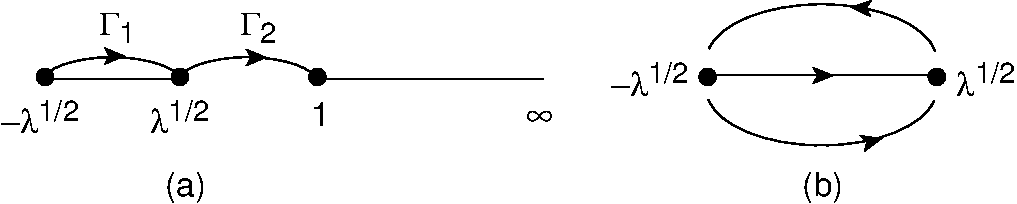
\includegraphics[width=0.95\textwidth]{figures/fig6.pdf}
  \caption{$\lambda$ 平面上的分支点与积分路径。(a) 分支点 $-\lambda^{1/2},\ \lambda^{1/2},\ 1,\ \infty$
           及路径 $\Gamma_1,\Gamma_2$；(b) 围绕 $\pm\lambda^{1/2}$ 的闭合路径及其定向。原文仅标
           “Figure 6”（原文 PDF 第 77 页），无说明性图注。}
  \label{fig:6}
\end{figure}

\begin{figure}[htbp]
  \centering
  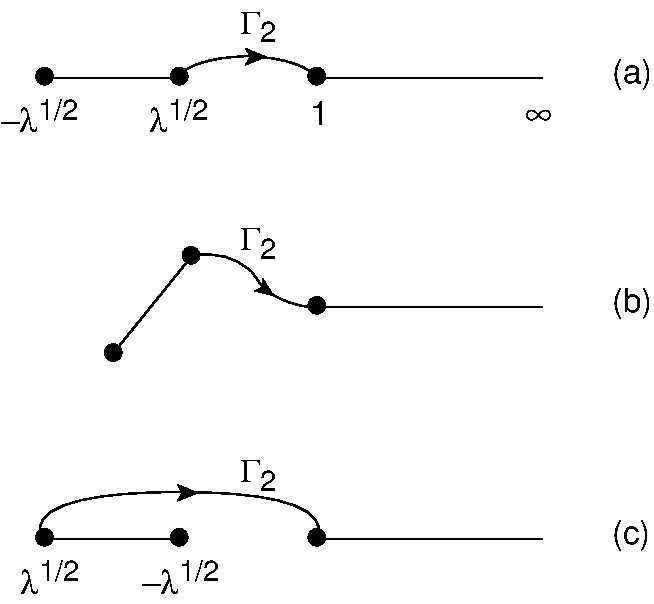
\includegraphics[width=0.55\textwidth]{figures/fig7.pdf}
  \caption{路径 $\Gamma_2$ 的变形。(a) $\lambda$ 平面上的 $\Gamma_2$；(b) 绕过分支点 $1$ 的变形；
           (c) 等价路径表示。原文仅标 “Figure 7”（原文 PDF 第 77 页），无说明性图注。}
  \label{fig:7}
\end{figure}

给定任意多项式，一个有用的量是它的判别式，定义为
$$
\Delta = \prod_{i<j} (e_i - e_j)^2,
$$
其中 $e_i$ 是根。$\Delta$ 可以用多项式的系数表达。显然，在两个分支点重合
的奇点处 $\Delta = 0$（$\infty$ 处的奇点除外）。例如对
$y^2 = (x-1)(x^2-u^n)$，在 $u = 0$ 附近 $\Delta \sim u^n$，而单值变换
共轭于 $T^n$。因此，在稳定情形下，单值变换的指数就是 $\Delta$ 的零点
阶数。例如，对由 (\ref{f2}) 描述的曲线族，$\Delta$ 在 $u=\pm\Lambda^2$
处有一阶零点，绕这些点的单值变换共轭于 $T$。
现在我们来看 $u\rightarrow \infty$。对大 $u$，分支点大约位于
$x=0,\,\Lambda^4/4u,\,u,\,\infty$。因此 $u=\infty$ 处的奇点不稳定，因为
在这一极限下多于两个分支点重合。这可以通过变量代换
$$
x = x'u\,, \qquad y = y' u^{3/2}\,,
$$
来修正，它把分支点移到 $0,\,\Lambda^4/4u^2,\,1,\,\infty$。判别式现在
表现为 $\Delta \sim u^{-4}$，对应共轭于 $T^{-4}$ 的单值变换。由于
$y \rightarrow y'$ 中存在 $\sqrt u$，用原来的变量 $(x,y)$ 表示时，单值
变换多出一个负号，共轭于 $PT^{-4}$。于是我们看到，曲线 (\ref{f2}) 给出
了 $N_f = 0$ 理论的正确单值变换。

% [Tutor Note: 见原文 PDF 第 77 页。$u\to\infty$ 处的奇点“不稳定”指
% 多于两个分支点重合。用 $x=x'u,\ y=y'u^{3/2}$ 把分支点移到有限位置后，
% 判别式在 $(x',y')$ 变量下表现为 $\Delta\sim u^{-4}$，对应共轭于
% $T^{-4}$ 的单值变换；但 $y=y'u^{3/2}$ 中的 $u^{3/2}$ 含有 $\sqrt u$，
% 绕 $u=0$ 一圈会给出额外的 $-1$，故回到原变量 $(x,y)$ 后单值变换是
% $PT^{-4}$ 而不是 $T^{-4}$（$P=-1$ 即宇称）。漏掉这个负号、把结果写成
% $T^{-4}$ 是最常见的错误。另外注意判别式的定义不含首项系数与整体符号，
% 与某些文献的约定相差常数因子。]

为了得到非零 $N_f$ 理论的曲线，我们应当知道这些理论中出现的单值变换。
这可以容易地算出来（如同 $N_f=0$ 情形），因为我们已经知道在 $u$ 平面
奇点处变为无质量的粒子的电荷谱。首先注意，如同 $N_f=0$ 理论，
$u=\infty$ 处的单值变换可以由微扰 $\beta$ 函数 (\ref{betanf})、或等价
地由 (\ref{betanf-mon}) 得到，结果为
$$
{\cal M}_{\infty} = PT^{N_f -4}.
$$
$u$ 平面有限点处的奇点一般对应无质量的磁单极，它们带一个单位的磁荷和
$n_e$ 个单位的电荷。为计算相应的单值变换，我们必须转到理论的对偶描述，
在其中磁单极与对偶规范场的耦合方式如同电子与通常规范场的耦合。在这一
框架下，单值变换由含 $k$ 个超多重态的单圈 QED $\beta$ 函数
(\ref{beta-hyper}) 决定，并由 $T^k$ 给出。这还必须与 $T^{n_e}S$ 共轭，
后者把荷为 $(0,1)$ 的超多重态变成荷为 $(1,n_e)$ 的磁单极。因此绕一个有
$k$ 个 $(n_m = 1, n_e)$ 磁单极的点的单值变换是
$(T^{n_e}S) T^k (T^{n_e}S)^{-1}$。类似的论证可用于计算 $N_f = 3$ 理论
中 $(2,1)$ 态的单值变换。下面我们列出上一小节描述的奇点周围的所有单值
变换：
$$
\begin{array}{rl}
N_f=0:& STS^{-1},\,(T^2 S)T(T^2 S)^{-1}\rightarrow M_{\infty}=PT^{-4}\,,\\
N_f=1:& STS^{-1},\,(TS)T(TS)^{-1},\, (T^2S)T(T^2S)^{-1} \rightarrow
M_{\infty}=PT^{-3}\,, \\
N_f=2:& ST^2 S^{-1},\,(TS)T^2(TS)^{-1}\rightarrow M_{\infty}=PT^{-2}\,,\\
N_f=3:& (ST^2S)T(ST^2S)^{-1},\,ST^4 S^{-1}\rightarrow
M_{\infty}=PT^{-1}\,. \\
\end{array}
$$
利用 $S^2=-1$ 与 $(ST)^3=1$，很容易验证对每个 $N_f$，有限 $u$ 处单值
矩阵的乘积都给出 $M_{\infty}$。注意在前三种情形（$N_f = 0,1,2$）中，
赋给奇点的电荷与我们先前论证所确定的电荷在符号上不同。这与把普适电荷和
群中心下的变换性质相联系时固有的不确定性一致。基于目前获得的知识，下面
我们概述 Seiberg 与 Witten 得到非零 $N_f$ 理论曲线显式形式的论证。

% [Tutor Note: 见原文 PDF 第 78 页。原文“massless magnetic monopoles with
% one unit of magnetic charge and $n_e$ units of magnetic charge”中第二个
% “magnetic charge”应为“electric charge”：磁单极带一个单位的磁荷与
% $n_e$ 个单位的电荷，这正是 $(n_m,n_e)=(1,n_e)$ 的含义。系原文笔误，
% 译文按正确含义（电荷）译出。另注意上表的单值矩阵之积给出
% $M_\infty=PT^{N_f-4}$，可用 $S^2=-1$、$(ST)^3=1$ 逐项核验；它是后面
% 确定各曲线形式的主要约束。]

\noindent\underline{$N_f =0$ 曲线的性质}：
在继续之前，列举 $N_f=0$ 曲线的一些性质非常有用，这些性质预期对非零
$N_f$ 仍然成立：
\begin{enumerate}
\item
描述曲线族的方程取一般形式 $y^2=F(x,u,\Lambda)$，其中 $F$ 是 $x$ 与 $u$
的不超过三次的多项式。
\item
$F$ 中关于 $x$ 与 $u$ 三次的部分是 $F_0 = x^2 (x-u)$。
\item
若给 $u$ 与 $x$ 赋 $U(1)_{\cal R}$ 荷 $4$、给 $\Lambda$ 赋荷 $2$，则
$F$ 的荷为 $12$。若给 $y$ 赋荷 $6$，则曲线在 $U(1)_{\cal R}$ 变换下
不变。
\item
$F$ 可以写成 $F = F_{0} + \Lambda^4 F_1$，其中 $F_1 = x/4$。
\end{enumerate}

性质 (1) 对 $N_f > 0$ 仍是一个拟设。它将给出正确的单值矩阵，并且在考虑
$N_f = 4$ 理论时也能部分地得到证明。性质 (2) 是下述事实的推论：当
$u \rightarrow \infty$ 时，我们必须得到与 $a_D$ 中来自单圈 $\beta$ 函数
的对数相联系的无穷远单值变换。这意味着有限 $x$ 处的某一个分支点应当在
$u\rightarrow\infty$ 时移到无穷远。对大 $u$，三次部分可以写成
$(x-e_1 u)(x-e_2 u)(x-e_3 u)$。于是，若两个 $e_i$ 相等而另一个不同（比如
$e_1=e_2\not=e_3$），就可得到所期望的行为。在这种情况下，通过重新定义
$x$，可以把 $F_0$ 化成 $x^2 (x-u)$ 的形式。性质 (4) 在 $N_f = 0$ 理论中
是 $U(1)_R$ 荷赋值的推论。注意 $F$ 只有一项经典贡献加上一项单瞬子项：
$\Lambda^4 x/4$。现在我们用这些性质来确定 $N_f = 1,2,3$ 的曲线。

\noindent\underline{无质量 $N_f=1$ 理论的曲线}：
在这个理论中，由方程 (\ref{inst-nf})，瞬子振幅正比于 $\Lambda^3_{1}$。
然而对 $N_f \geq 1$，瞬子因子在 $\rho$ 宇称下为奇，因此 $F$ 中只能出现
它的偶次幂。由于 $\Lambda_{1}$ 的 $U(1)_R$ 荷为 $2$、$F$ 的荷为 $12$，
唯一的可能是
$$
y^2 = x^2 (x-u) + t \Lambda^{6}_{1} \,.
$$
常数 $t$ 可以吸收到 $\Lambda_{1}$ 的重定义中：
$t\Lambda^{6}_{1}=\tilde{\Lambda}^6$。这一曲线族的判别式为
$$
\Delta = \tilde{\Lambda}^{6}_{1} (4 u^3 - 27 \tilde{\Lambda}^{6}_{1})\,.
$$
它有三个零点，这些零点在作用在 $u$ 平面上的 ${\bf Z}_3$ 变换下互相
交换，相应的单值变换共轭于 $T$。类似地，大 $u$ 处的单值变换可以算出为
$PT^{-3}$。这与 $N_f=1$ 理论应有的结果一致。

% [Tutor Note: 见原文 PDF 第 79 页。可用三次式 $x^3-ux^2+\tilde\Lambda^6$
% 的判别式 $\Delta=4u^3\tilde\Lambda^6-27\tilde\Lambda^{12}$ 核验此式：
% $x^3+ax^2+bx+c$ 的判别式为 $a^2b^2-4b^3-4a^3c-27c^2+18abc$，代入
% $a=-u,\ b=0,\ c=\tilde\Lambda^6$ 即得。注意原文的 $\Delta$ 定义不含
% 首项系数，与某些文献相差一个常数因子；零点位置（$u^3=\frac{27}{4}
% \tilde\Lambda^6$，三个零点相差 ${\bf Z}_3$ 相位）才是物理上重要的。]

\noindent\underline{无质量 $N_f=2$ 理论的曲线}：
在这种情况下瞬子因子是 $\Lambda^{2}_{2}$，同样，在没有裸质量时，$F$ 中
只能出现它的偶次幂。由于 $\Lambda_2$ 的 $U(1)_R$ 荷为 2，曲线的一般形式为
$$
y^2 = x^2 (x-u) + (ax + bu) \Lambda^{4}_{2}\,.
$$
根据我们对 $N_f=2$ 理论的讨论，预期有两个奇点，每个奇点带两个无质量磁单极。
因此每个奇点处的单值变换共轭于 $T^2$，这意味着每个有限奇点处的判别式
应当有二阶零点。这一条件确定了 $a$ 与 $b$。在对 $\Lambda_2$ 作重新标度
之后，$N_f=2$ 曲线族可以写成
$$
y^2 = (x^2 - \tilde{\Lambda}^{4}_{2} ) (x-u)\,,
$$
它具有所预期的 ${\bf Z}_2$ 对称性。

% [Tutor Note: 见原文 PDF 第 79 页。注意 $(x^2-\tilde\Lambda_2^4)(x-u)
% = x^3-ux^2-\tilde\Lambda_2^4x+u\tilde\Lambda_2^4$ 确实具有上式的
% “$(ax+bu)\Lambda_2^4$”形式：$a=-1,\ b=1$。所谓“判别式在每个有限奇点
% 处有二阶零点”即 $\Delta$ 有两个二重零点（对应两个奇点各两个无质量
% 单极），这正好确定两个系数 $a,b$。原文省略了这一代数步骤。]

\noindent\underline{无质量 $N_f=3$ 理论的曲线}：
在这种情况下，$u$ 平面上有两个奇点，其单值变换分别共轭于 $T^4$ 与 $T$，
并且没有对称性作用在 $u$ 平面上。取 $T^4$ 奇点在 $u = 0$。于是判别式
应在 $u=0$ 处有四阶零点。这与通常的 $U(1)_{\cal R}$ 荷及 $\rho$ 宇称
赋值一起给出
$$
F = a \Lambda^{2}_{3} x^2 + bu^2 x + cu x^2 + x^3 \,.
$$
这里 $b \not= 0$，否则曲线对所有 $u$ 都是奇异的。要求 $F$ 的三次部分
具有所期望的经典行为，并经过一些重新标度后，得到
$$
y^2 = x^2 (x-u) + \tilde {\Lambda}^{2}_{3} (x-u)^2\,.
$$

% [Tutor Note: 见原文 PDF 第 79--80 页。原文只给出拟设与最终曲线，中间
% “要求三次部分具有经典行为”和“经过一些重新标度”两步完全没有展开：
% 由 $F=x^3+(a\Lambda_3^2+cu)x^2+bu^2x$ 算判别式可得
% $\Delta=b^2u^4[(a\Lambda_3^2+cu)^2-4bu^2]$，在 $u=0$ 处的四阶零点由
% $b^2u^4$ 自动给出（$b\ne0$），这解释了下文“$b\not=0$”的条件；而
% $x$、$y$ 的允许重参数化（含 $x$ 的平移/标度）会把拟设化为最终形式。
% 原文未展示这些步骤，若需复现请参看 [32] 的严格处理。]

注意上面我们只考虑了没有裸质量项的理论。由于质量项具有奇的 $\rho$-宇称，
在有非零裸质量的理论中，瞬子因子的奇次幂也可以对曲线方程有贡献。我们在此
不讨论这些情形，但为完整起见，直接列出最终结果：
\begin{eqnarray}
N_f=1:\qquad y^2 &=& x^2(x-u)+ \frac{1}{4}m\Lambda_1^3 x -
\frac{1}{64} \Lambda_1^6\,, \nonumber \\
N_f=2:\qquad y^2 &=& (x^2-\frac{1}{64}\Lambda_2^4) (x-u) + m_1 m_2
\Lambda_2^2 x - \frac{1}{64}(m_1^2+m_2^2)\Lambda_2^4\,,\nonumber \\
N_f=3:\qquad y^2 &=& x^2(x-u)-\frac{1}{64} \Lambda_3^2(x-u)^2
-\frac{1}{64}(m_1^2+m_2^2+m_3^2) \Lambda_3^2(x-u) \nonumber \\
      && +\frac{1}{4}m_1m_2m_3 \Lambda_3 x - \frac{1}{64}
(m_1^2 m_2^2 + m_2^2 m_3^2 + m_1^2 m_3^2)\Lambda_3^2\,. \nonumber
\end{eqnarray}
关于更多细节与讨论（包括 $N_f=4$ 情形），以及得到曲线方程的更严格方法，
读者可参阅 Seiberg 与 Witten 的原始工作 \cite{SW2}。

% [Tutor Note: 见原文 PDF 第 80 页。这三条曲线在原书中全部带 nonumber
% 标注，因此不占公式编号，但它们与前面无质量曲线的关系可以
% 逐项核验：$m_i\to0$ 时 $N_f=1$ 给出 $-\frac1{64}\Lambda_1^6$（对应
% $t=-1/64$），$N_f=2$ 给出 $(x^2-\frac1{64}\Lambda_2^4)(x-u)$（对应
% $\tilde\Lambda_2^4=\frac1{64}\Lambda_2^4$），$N_f=3$ 给出
% $-\frac1{64}\Lambda_3^2(x-u)^2$（对应
% $\tilde\Lambda_3^2=-\frac1{64}\Lambda_3^2$，故 $\tilde\Lambda_3^2$
% 的符号与 $\Lambda_3^2$ 相反）。核对符号时以这一极限为依据。]

一旦曲线确定，其余步骤就与 $N_f=0$ 情形非常相似。我们通过围道积分定义
量 $a$ 与 $a_D$：
$$
a=\int_{\gamma_1} \, \lambda\,,\quad a_D=\int_{\gamma_2}\lambda\,,
$$
度规由 ${\rm Im}(\tau)$ 给出，其中 $\tau=\frac{da_D}{du}/
\frac{da}{du}$。这里 $\lambda$ 是一个全纯一形式，满足
$$ 
\frac{d\lambda}{du}=\frac{\sqrt 2}{8\pi}\frac{dx}{y}\,.
$$
与 $N_f=0$ 情形的差别在于，现在 $\lambda$ 可以有非零留数的极点，不过
留数应当与 $u$ 无关。若如此，则 $\tau$ 仍经历 $SL(2,Z)$ 变换，而
$(a_D, a)$ 经历 $SL(2,Z)$ 变换外加一个移动。正如我们在带非零裸质量夸克的
QED 情形所看到的，这一移动实际上是必需的，并且与修改后的 BPS 质量公式
(\ref{bps-m}) 一致。由此推出，造成移动的 $\lambda$ 的留数应当正比于裸
夸克质量。这一点已在 \cite{SW2} 中对 $N_f=2$ 曲线作了检验，并发现确实
如此。事实上，留数的存在具有很强的限制性，Seiberg 与 Witten 正是利用
这一信息以严格的方式导出了 $N_f=4$ 理论的曲线。其他理论的曲线则可以由
重整化群流确定，结果与上面所列一致。

% [Tutor Note: 见原文 PDF 第 80 页。$d\lambda/du$ 的系数
% $\sqrt2/(8\pi)$ 中含因子 $\sqrt2$ 与 $8\pi$，与式 (109)
% 的 $1/2\pi$、式 (111) 的 $1/16\pi^2$ 相互关联；改动任何一处
% 归一化都会破坏周期 $a,a_D$ 与单值矩阵的一致性，抄写时必须逐字符核对。
% 另外原文“used by Seiberg and Witten to drive the curve”中的“drive”
% 系“derive”（导出）的拼写笔误；同页“varialbles”（应为 variables）、
% “form the perturbative”（应为 from）等亦为排印笔误。全片类似的拼写
% 笔误还有 sigularities（应为 singularities，第 74--75 页）、
% analoguous（应为 analogous，第 73 页）、representaion（应为
% representation，第 73 页），译文均已按正确词义处理。留数正比于裸质量
% 是本节与前面 QED 讨论（$a_D$ 的平移）相呼应的关键结论。]

